% Options for packages loaded elsewhere
\PassOptionsToPackage{unicode}{hyperref}
\PassOptionsToPackage{hyphens}{url}
%
\documentclass[
]{article}
\usepackage{amsmath,amssymb}
\usepackage{iftex}
\ifPDFTeX
  \usepackage[T1]{fontenc}
  \usepackage[utf8]{inputenc}
  \usepackage{textcomp} % provide euro and other symbols
\else % if luatex or xetex
  \usepackage{unicode-math} % this also loads fontspec
  \defaultfontfeatures{Scale=MatchLowercase}
  \defaultfontfeatures[\rmfamily]{Ligatures=TeX,Scale=1}
\fi
\usepackage{lmodern}
\ifPDFTeX\else
  % xetex/luatex font selection
\fi
% Use upquote if available, for straight quotes in verbatim environments
\IfFileExists{upquote.sty}{\usepackage{upquote}}{}
\IfFileExists{microtype.sty}{% use microtype if available
  \usepackage[]{microtype}
  \UseMicrotypeSet[protrusion]{basicmath} % disable protrusion for tt fonts
}{}
\makeatletter
\@ifundefined{KOMAClassName}{% if non-KOMA class
  \IfFileExists{parskip.sty}{%
    \usepackage{parskip}
  }{% else
    \setlength{\parindent}{0pt}
    \setlength{\parskip}{6pt plus 2pt minus 1pt}}
}{% if KOMA class
  \KOMAoptions{parskip=half}}
\makeatother
\usepackage{xcolor}
\usepackage[margin=1in]{geometry}
\usepackage{color}
\usepackage{fancyvrb}
\newcommand{\VerbBar}{|}
\newcommand{\VERB}{\Verb[commandchars=\\\{\}]}
\DefineVerbatimEnvironment{Highlighting}{Verbatim}{commandchars=\\\{\}}
% Add ',fontsize=\small' for more characters per line
\usepackage{framed}
\definecolor{shadecolor}{RGB}{248,248,248}
\newenvironment{Shaded}{\begin{snugshade}}{\end{snugshade}}
\newcommand{\AlertTok}[1]{\textcolor[rgb]{0.94,0.16,0.16}{#1}}
\newcommand{\AnnotationTok}[1]{\textcolor[rgb]{0.56,0.35,0.01}{\textbf{\textit{#1}}}}
\newcommand{\AttributeTok}[1]{\textcolor[rgb]{0.13,0.29,0.53}{#1}}
\newcommand{\BaseNTok}[1]{\textcolor[rgb]{0.00,0.00,0.81}{#1}}
\newcommand{\BuiltInTok}[1]{#1}
\newcommand{\CharTok}[1]{\textcolor[rgb]{0.31,0.60,0.02}{#1}}
\newcommand{\CommentTok}[1]{\textcolor[rgb]{0.56,0.35,0.01}{\textit{#1}}}
\newcommand{\CommentVarTok}[1]{\textcolor[rgb]{0.56,0.35,0.01}{\textbf{\textit{#1}}}}
\newcommand{\ConstantTok}[1]{\textcolor[rgb]{0.56,0.35,0.01}{#1}}
\newcommand{\ControlFlowTok}[1]{\textcolor[rgb]{0.13,0.29,0.53}{\textbf{#1}}}
\newcommand{\DataTypeTok}[1]{\textcolor[rgb]{0.13,0.29,0.53}{#1}}
\newcommand{\DecValTok}[1]{\textcolor[rgb]{0.00,0.00,0.81}{#1}}
\newcommand{\DocumentationTok}[1]{\textcolor[rgb]{0.56,0.35,0.01}{\textbf{\textit{#1}}}}
\newcommand{\ErrorTok}[1]{\textcolor[rgb]{0.64,0.00,0.00}{\textbf{#1}}}
\newcommand{\ExtensionTok}[1]{#1}
\newcommand{\FloatTok}[1]{\textcolor[rgb]{0.00,0.00,0.81}{#1}}
\newcommand{\FunctionTok}[1]{\textcolor[rgb]{0.13,0.29,0.53}{\textbf{#1}}}
\newcommand{\ImportTok}[1]{#1}
\newcommand{\InformationTok}[1]{\textcolor[rgb]{0.56,0.35,0.01}{\textbf{\textit{#1}}}}
\newcommand{\KeywordTok}[1]{\textcolor[rgb]{0.13,0.29,0.53}{\textbf{#1}}}
\newcommand{\NormalTok}[1]{#1}
\newcommand{\OperatorTok}[1]{\textcolor[rgb]{0.81,0.36,0.00}{\textbf{#1}}}
\newcommand{\OtherTok}[1]{\textcolor[rgb]{0.56,0.35,0.01}{#1}}
\newcommand{\PreprocessorTok}[1]{\textcolor[rgb]{0.56,0.35,0.01}{\textit{#1}}}
\newcommand{\RegionMarkerTok}[1]{#1}
\newcommand{\SpecialCharTok}[1]{\textcolor[rgb]{0.81,0.36,0.00}{\textbf{#1}}}
\newcommand{\SpecialStringTok}[1]{\textcolor[rgb]{0.31,0.60,0.02}{#1}}
\newcommand{\StringTok}[1]{\textcolor[rgb]{0.31,0.60,0.02}{#1}}
\newcommand{\VariableTok}[1]{\textcolor[rgb]{0.00,0.00,0.00}{#1}}
\newcommand{\VerbatimStringTok}[1]{\textcolor[rgb]{0.31,0.60,0.02}{#1}}
\newcommand{\WarningTok}[1]{\textcolor[rgb]{0.56,0.35,0.01}{\textbf{\textit{#1}}}}
\usepackage{graphicx}
\makeatletter
\def\maxwidth{\ifdim\Gin@nat@width>\linewidth\linewidth\else\Gin@nat@width\fi}
\def\maxheight{\ifdim\Gin@nat@height>\textheight\textheight\else\Gin@nat@height\fi}
\makeatother
% Scale images if necessary, so that they will not overflow the page
% margins by default, and it is still possible to overwrite the defaults
% using explicit options in \includegraphics[width, height, ...]{}
\setkeys{Gin}{width=\maxwidth,height=\maxheight,keepaspectratio}
% Set default figure placement to htbp
\makeatletter
\def\fps@figure{htbp}
\makeatother
\setlength{\emergencystretch}{3em} % prevent overfull lines
\providecommand{\tightlist}{%
  \setlength{\itemsep}{0pt}\setlength{\parskip}{0pt}}
\setcounter{secnumdepth}{-\maxdimen} % remove section numbering
\ifLuaTeX
  \usepackage{selnolig}  % disable illegal ligatures
\fi
\IfFileExists{bookmark.sty}{\usepackage{bookmark}}{\usepackage{hyperref}}
\IfFileExists{xurl.sty}{\usepackage{xurl}}{} % add URL line breaks if available
\urlstyle{same}
\hypersetup{
  pdftitle={Compare Experiment Conditions Cohort1},
  pdfauthor={Sean Maden},
  hidelinks,
  pdfcreator={LaTeX via pandoc}}

\title{Compare Experiment Conditions Cohort1}
\author{Sean Maden}
\date{2023-08-28}

\begin{document}
\maketitle

\hypertarget{setup-experiment-parameters}{%
\section{Setup experiment
parameters}\label{setup-experiment-parameters}}

\hypertarget{k2-results}{%
\section{1. K2 results}\label{k2-results}}

Set up the snRNAseq data with K markers.

\hypertarget{experiment-1a.}{%
\subsection{Experiment 1A.}\label{experiment-1a.}}

\begin{itemize}
\tightlist
\item
  \(P_{true}\) : RNAscope proportions, grouped by \texttt{sample.id}.
\item
  \(G\) : Batch-robust markers from training (\(N\) = 20 genes per
  celltype \(k\)).
\item
  \(Z\) : Matched or unmatched expression, grouped by
  \texttt{sample.id}.
\item
  \(S\) : Tests sizes from RNAscope cell sizes, grouped by
  \texttt{sample.id}.
\end{itemize}

\hypertarget{summarize-matched-rnascope-sizes-results-train}{%
\subsection{Summarize matched RNAscope sizes results --
train}\label{summarize-matched-rnascope-sizes-results-train}}

Tabular results summary

\hypertarget{export-env}{%
\section{Export env}\label{export-env}}

\hypertarget{results}{%
\section{Results}\label{results}}

\begin{Shaded}
\begin{Highlighting}[]
\CommentTok{\# load env with plot entities}
\FunctionTok{setwd}\NormalTok{(}\StringTok{".."}\NormalTok{)}
\FunctionTok{setwd}\NormalTok{(}\StringTok{".."}\NormalTok{)}
\NormalTok{env.name }\OtherTok{\textless{}{-}} \StringTok{"02\_notebook.RData"}
\NormalTok{env.path }\OtherTok{\textless{}{-}} \FunctionTok{file.path}\NormalTok{(}\StringTok{"outputs"}\NormalTok{, }\StringTok{"14\_compare{-}expt{-}conditions{-}cohort1"}\NormalTok{, env.name)}
\FunctionTok{load}\NormalTok{(}\AttributeTok{file=}\NormalTok{env.path)}
\end{Highlighting}
\end{Shaded}

\hypertarget{boxplots}{%
\subsection{Boxplots}\label{boxplots}}

\hypertarget{training-results}{%
\subsubsection{Training results}\label{training-results}}

Training summaries by sample id, treatment

\begin{Shaded}
\begin{Highlighting}[]
\NormalTok{df.res.filt }\OtherTok{\textless{}{-}}\NormalTok{ df.res[df.res}\SpecialCharTok{$}\NormalTok{sample.id }\SpecialCharTok{==}\NormalTok{ df.res}\SpecialCharTok{$}\NormalTok{dfs.rn.sample.id,]}
\FunctionTok{dim}\NormalTok{(df.res.filt)}
\end{Highlighting}
\end{Shaded}

\begin{verbatim}
## [1] 60 18
\end{verbatim}

\begin{Shaded}
\begin{Highlighting}[]
\CommentTok{\# get facet summaries}
\FunctionTok{ggplot}\NormalTok{(df.res.filt, }\FunctionTok{aes}\NormalTok{(}\AttributeTok{x =}\NormalTok{ experiment.type, }
                        \AttributeTok{y =}\NormalTok{ error.neuron.true.pred, }\AttributeTok{color =}\NormalTok{ sample.id)) }\SpecialCharTok{+} \FunctionTok{geom\_jitter}\NormalTok{(}\AttributeTok{alpha =} \FloatTok{0.5}\NormalTok{) }\SpecialCharTok{+} 
  \FunctionTok{geom\_boxplot}\NormalTok{(}\AttributeTok{alpha =} \DecValTok{0}\NormalTok{, }\AttributeTok{color =} \StringTok{"cyan"}\NormalTok{) }\SpecialCharTok{+} \FunctionTok{xlab}\NormalTok{(}\StringTok{"Z reference type"}\NormalTok{) }\SpecialCharTok{+}
  \FunctionTok{ggtitle}\NormalTok{(}\StringTok{"S RNAscope matched"}\NormalTok{) }\SpecialCharTok{+} \FunctionTok{facet\_wrap}\NormalTok{(}\SpecialCharTok{\textasciitilde{}}\NormalTok{y.expt.condition)}
\end{Highlighting}
\end{Shaded}

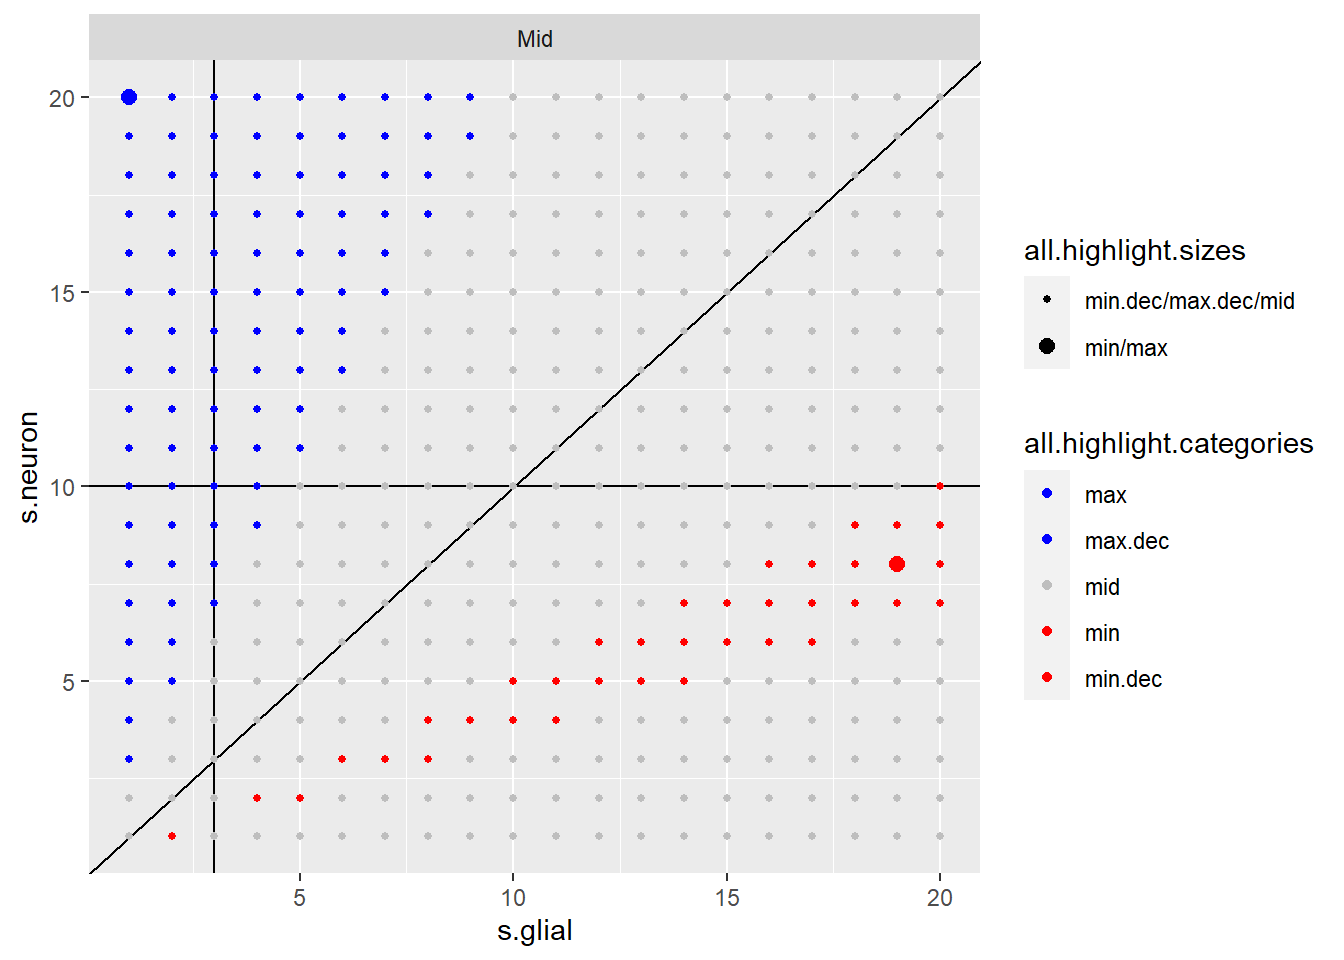
\includegraphics{02_only-rnascope-sizes_compare-experiment-conditions-cohort1_files/figure-latex/unnamed-chunk-9-1.pdf}

\begin{Shaded}
\begin{Highlighting}[]
\FunctionTok{ggplot}\NormalTok{(df.res.filt, }\FunctionTok{aes}\NormalTok{(}\AttributeTok{x =}\NormalTok{ experiment.type, }
                        \AttributeTok{y =}\NormalTok{ error.neuron.true.pred, }\AttributeTok{color =}\NormalTok{ sample.id)) }\SpecialCharTok{+} \FunctionTok{geom\_jitter}\NormalTok{(}\AttributeTok{alpha =} \FloatTok{0.5}\NormalTok{) }\SpecialCharTok{+} 
  \FunctionTok{geom\_boxplot}\NormalTok{(}\AttributeTok{alpha =} \DecValTok{0}\NormalTok{, }\AttributeTok{color =} \StringTok{"cyan"}\NormalTok{) }\SpecialCharTok{+} \FunctionTok{xlab}\NormalTok{(}\StringTok{"Z reference type"}\NormalTok{) }\SpecialCharTok{+}
  \FunctionTok{ggtitle}\NormalTok{(}\StringTok{"S RNAscope matched"}\NormalTok{) }\SpecialCharTok{+} \FunctionTok{facet\_wrap}\NormalTok{(}\SpecialCharTok{\textasciitilde{}}\NormalTok{cell.compartment)}
\end{Highlighting}
\end{Shaded}

\includegraphics{02_only-rnascope-sizes_compare-experiment-conditions-cohort1_files/figure-latex/unnamed-chunk-9-2.pdf}

\begin{Shaded}
\begin{Highlighting}[]
\FunctionTok{ggplot}\NormalTok{(df.res.filt, }\FunctionTok{aes}\NormalTok{(}\AttributeTok{x =}\NormalTok{ experiment.type, }
                        \AttributeTok{y =}\NormalTok{ error.neuron.true.pred, }\AttributeTok{color =}\NormalTok{ sample.id)) }\SpecialCharTok{+} \FunctionTok{geom\_jitter}\NormalTok{(}\AttributeTok{alpha =} \FloatTok{0.5}\NormalTok{) }\SpecialCharTok{+} 
  \FunctionTok{geom\_boxplot}\NormalTok{(}\AttributeTok{alpha =} \DecValTok{0}\NormalTok{, }\AttributeTok{color =} \StringTok{"cyan"}\NormalTok{) }\SpecialCharTok{+} \FunctionTok{xlab}\NormalTok{(}\StringTok{"Z reference type"}\NormalTok{) }\SpecialCharTok{+}
  \FunctionTok{ggtitle}\NormalTok{(}\StringTok{"S RNAscope matched"}\NormalTok{) }\SpecialCharTok{+} \FunctionTok{facet\_wrap}\NormalTok{(}\SpecialCharTok{\textasciitilde{}}\NormalTok{library.type)}
\end{Highlighting}
\end{Shaded}

\includegraphics{02_only-rnascope-sizes_compare-experiment-conditions-cohort1_files/figure-latex/unnamed-chunk-9-3.pdf}

\begin{Shaded}
\begin{Highlighting}[]
\FunctionTok{ggplot}\NormalTok{(df.res.filt, }\FunctionTok{aes}\NormalTok{(}\AttributeTok{x =}\NormalTok{ experiment.type, }
                        \AttributeTok{y =}\NormalTok{ error.neuron.true.pred, }\AttributeTok{color =}\NormalTok{ sample.id)) }\SpecialCharTok{+} \FunctionTok{geom\_jitter}\NormalTok{(}\AttributeTok{alpha =} \FloatTok{0.5}\NormalTok{) }\SpecialCharTok{+} 
  \FunctionTok{geom\_boxplot}\NormalTok{(}\AttributeTok{alpha =} \DecValTok{0}\NormalTok{, }\AttributeTok{color =} \StringTok{"cyan"}\NormalTok{) }\SpecialCharTok{+} \FunctionTok{xlab}\NormalTok{(}\StringTok{"Z reference type"}\NormalTok{) }\SpecialCharTok{+}
  \FunctionTok{ggtitle}\NormalTok{(}\StringTok{"S RNAscope matched"}\NormalTok{) }\SpecialCharTok{+} \FunctionTok{facet\_wrap}\NormalTok{(}\SpecialCharTok{\textasciitilde{}}\NormalTok{sample.id)}
\end{Highlighting}
\end{Shaded}

\includegraphics{02_only-rnascope-sizes_compare-experiment-conditions-cohort1_files/figure-latex/unnamed-chunk-9-4.pdf}

Training summaries by sample id

\begin{Shaded}
\begin{Highlighting}[]
\NormalTok{dft }\OtherTok{\textless{}{-}} \FunctionTok{aggregate}\NormalTok{(error.neuron.true.pred}\SpecialCharTok{\textasciitilde{}}\NormalTok{sample.id}\SpecialCharTok{*}\NormalTok{experiment.type, }\AttributeTok{data =}\NormalTok{ df.res.filt, }\AttributeTok{FUN =} \StringTok{"median"}\NormalTok{)}
\FunctionTok{colnames}\NormalTok{(dft)[}\DecValTok{3}\NormalTok{] }\OtherTok{\textless{}{-}} \FunctionTok{paste0}\NormalTok{(}\StringTok{"median."}\NormalTok{, }\FunctionTok{colnames}\NormalTok{(dft)[}\DecValTok{3}\NormalTok{])}

\FunctionTok{ggplot}\NormalTok{(dft, }\FunctionTok{aes}\NormalTok{(}\AttributeTok{x =}\NormalTok{ experiment.type, }
                \AttributeTok{y =}\NormalTok{ median.error.neuron.true.pred, }\AttributeTok{color =}\NormalTok{ sample.id)) }\SpecialCharTok{+} \FunctionTok{geom\_jitter}\NormalTok{(}\AttributeTok{alpha =} \FloatTok{0.5}\NormalTok{) }\SpecialCharTok{+} 
  \FunctionTok{geom\_boxplot}\NormalTok{(}\AttributeTok{alpha =} \DecValTok{0}\NormalTok{, }\AttributeTok{color =} \StringTok{"cyan"}\NormalTok{) }\SpecialCharTok{+} \FunctionTok{xlab}\NormalTok{(}\StringTok{"Z reference type"}\NormalTok{) }\SpecialCharTok{+} \FunctionTok{ggtitle}\NormalTok{(}\StringTok{"S RNAscope matched"}\NormalTok{)}
\end{Highlighting}
\end{Shaded}

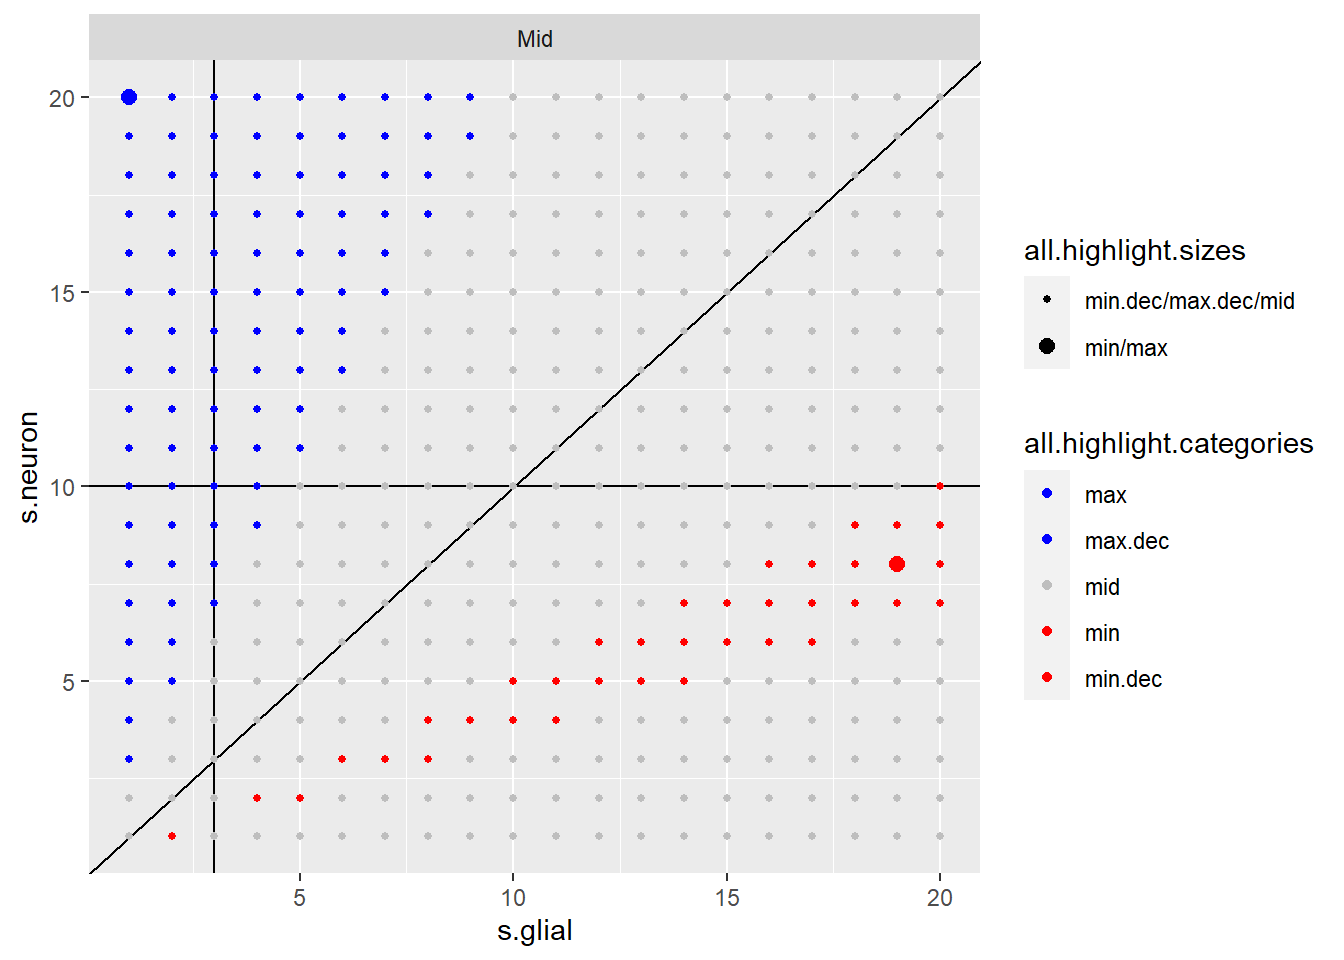
\includegraphics{02_only-rnascope-sizes_compare-experiment-conditions-cohort1_files/figure-latex/unnamed-chunk-10-1.pdf}

\hypertarget{validation-results}{%
\subsubsection{Validation results}\label{validation-results}}

Validation summaries by sample id, treatment

\begin{Shaded}
\begin{Highlighting}[]
\NormalTok{df.res.filt }\OtherTok{\textless{}{-}}\NormalTok{ df.res[df.res}\SpecialCharTok{$}\NormalTok{sample.id }\SpecialCharTok{==}\NormalTok{ df.res}\SpecialCharTok{$}\NormalTok{dfs.rn.sample.id,]}
\FunctionTok{dim}\NormalTok{(df.res.filt)}
\end{Highlighting}
\end{Shaded}

\begin{verbatim}
## [1] 60 18
\end{verbatim}

\begin{Shaded}
\begin{Highlighting}[]
\CommentTok{\# get facet summaries}
\FunctionTok{ggplot}\NormalTok{(df.res.filt, }\FunctionTok{aes}\NormalTok{(}\AttributeTok{x =}\NormalTok{ experiment.type, }
                        \AttributeTok{y =}\NormalTok{ error.neuron.true.pred, }\AttributeTok{color =}\NormalTok{ sample.id)) }\SpecialCharTok{+} \FunctionTok{geom\_jitter}\NormalTok{(}\AttributeTok{alpha =} \FloatTok{0.5}\NormalTok{) }\SpecialCharTok{+} 
  \FunctionTok{geom\_boxplot}\NormalTok{(}\AttributeTok{alpha =} \DecValTok{0}\NormalTok{, }\AttributeTok{color =} \StringTok{"cyan"}\NormalTok{) }\SpecialCharTok{+} \FunctionTok{xlab}\NormalTok{(}\StringTok{"Z reference type"}\NormalTok{) }\SpecialCharTok{+}
  \FunctionTok{ggtitle}\NormalTok{(}\StringTok{"S RNAscope matched"}\NormalTok{) }\SpecialCharTok{+} \FunctionTok{facet\_wrap}\NormalTok{(}\SpecialCharTok{\textasciitilde{}}\NormalTok{y.expt.condition)}
\end{Highlighting}
\end{Shaded}

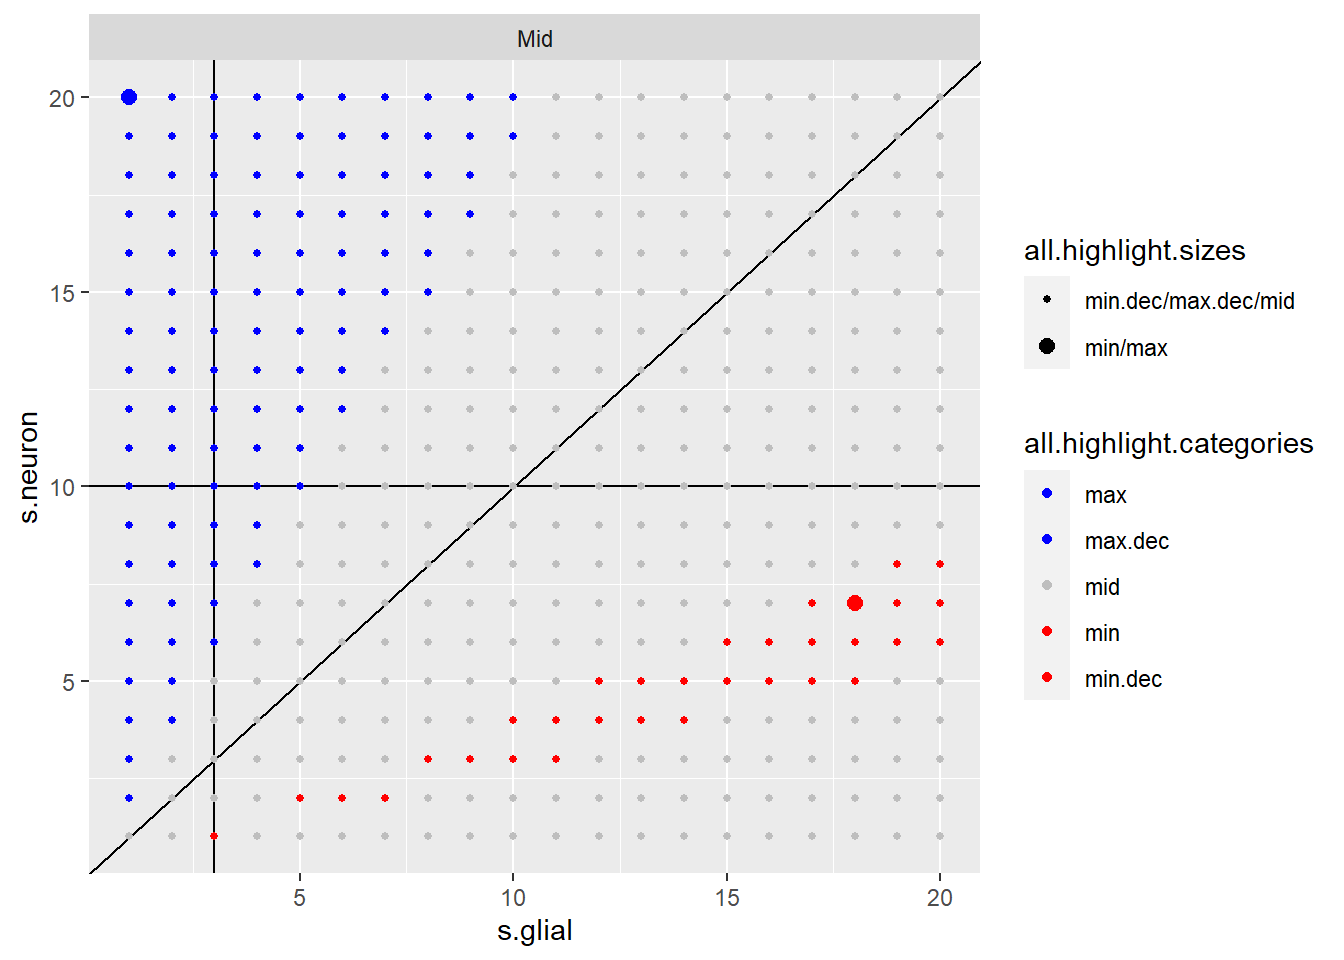
\includegraphics{02_only-rnascope-sizes_compare-experiment-conditions-cohort1_files/figure-latex/unnamed-chunk-11-1.pdf}

\begin{Shaded}
\begin{Highlighting}[]
\FunctionTok{ggplot}\NormalTok{(df.res.filt, }\FunctionTok{aes}\NormalTok{(}\AttributeTok{x =}\NormalTok{ experiment.type, }
                        \AttributeTok{y =}\NormalTok{ error.neuron.true.pred, }\AttributeTok{color =}\NormalTok{ sample.id)) }\SpecialCharTok{+} \FunctionTok{geom\_jitter}\NormalTok{(}\AttributeTok{alpha =} \FloatTok{0.5}\NormalTok{) }\SpecialCharTok{+} 
  \FunctionTok{geom\_boxplot}\NormalTok{(}\AttributeTok{alpha =} \DecValTok{0}\NormalTok{, }\AttributeTok{color =} \StringTok{"cyan"}\NormalTok{) }\SpecialCharTok{+} \FunctionTok{xlab}\NormalTok{(}\StringTok{"Z reference type"}\NormalTok{) }\SpecialCharTok{+}
  \FunctionTok{ggtitle}\NormalTok{(}\StringTok{"S RNAscope matched"}\NormalTok{) }\SpecialCharTok{+} \FunctionTok{facet\_wrap}\NormalTok{(}\SpecialCharTok{\textasciitilde{}}\NormalTok{cell.compartment)}
\end{Highlighting}
\end{Shaded}

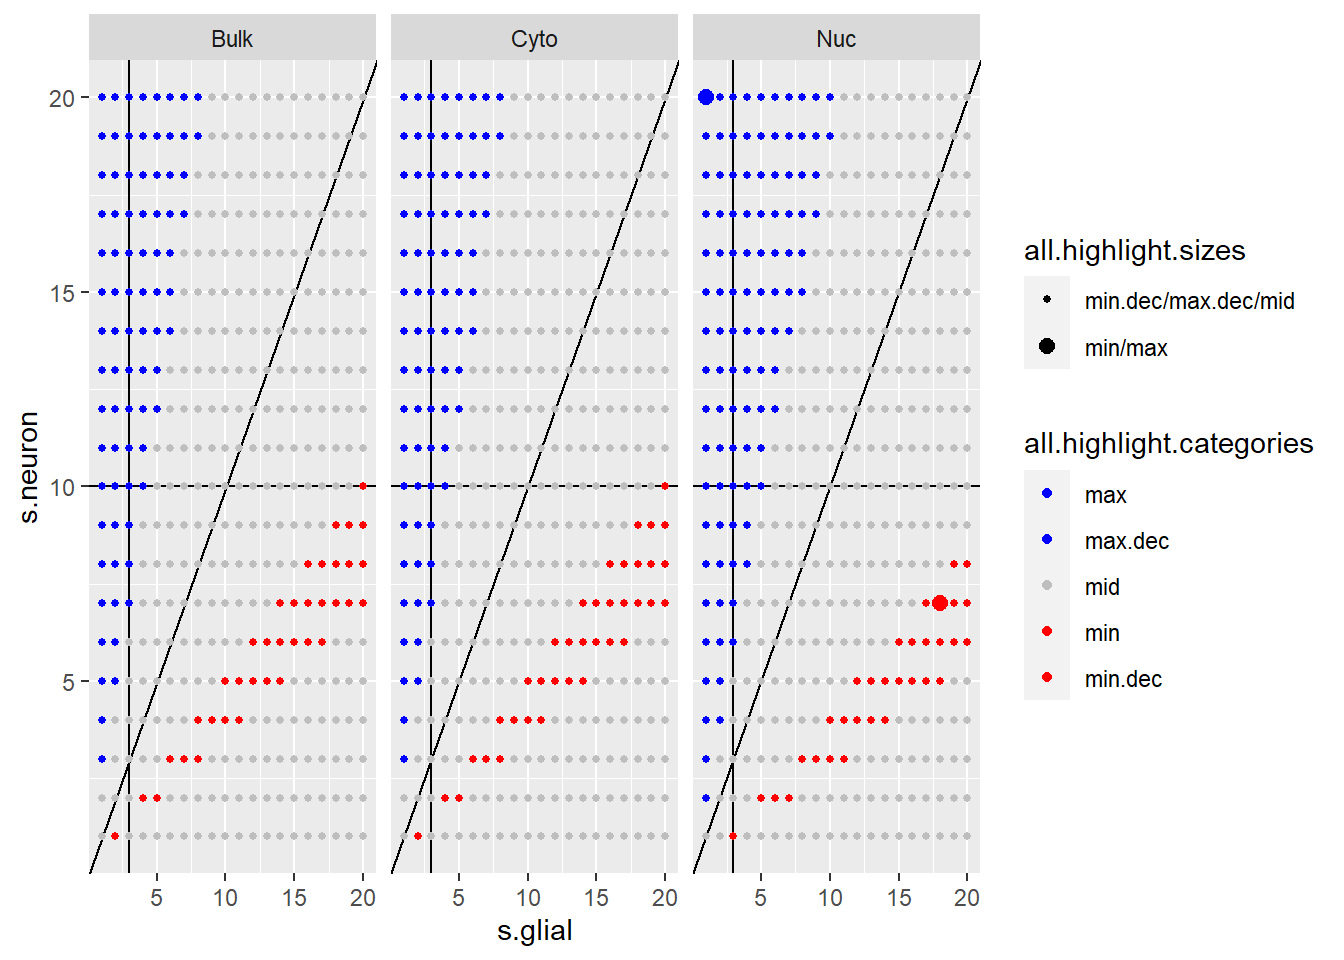
\includegraphics{02_only-rnascope-sizes_compare-experiment-conditions-cohort1_files/figure-latex/unnamed-chunk-11-2.pdf}

\begin{Shaded}
\begin{Highlighting}[]
\FunctionTok{ggplot}\NormalTok{(df.res.filt, }\FunctionTok{aes}\NormalTok{(}\AttributeTok{x =}\NormalTok{ experiment.type, }
                        \AttributeTok{y =}\NormalTok{ error.neuron.true.pred, }\AttributeTok{color =}\NormalTok{ sample.id)) }\SpecialCharTok{+} \FunctionTok{geom\_jitter}\NormalTok{(}\AttributeTok{alpha =} \FloatTok{0.5}\NormalTok{) }\SpecialCharTok{+} 
  \FunctionTok{geom\_boxplot}\NormalTok{(}\AttributeTok{alpha =} \DecValTok{0}\NormalTok{, }\AttributeTok{color =} \StringTok{"cyan"}\NormalTok{) }\SpecialCharTok{+} \FunctionTok{xlab}\NormalTok{(}\StringTok{"Z reference type"}\NormalTok{) }\SpecialCharTok{+}
  \FunctionTok{ggtitle}\NormalTok{(}\StringTok{"S RNAscope matched"}\NormalTok{) }\SpecialCharTok{+} \FunctionTok{facet\_wrap}\NormalTok{(}\SpecialCharTok{\textasciitilde{}}\NormalTok{library.type)}
\end{Highlighting}
\end{Shaded}

\includegraphics{02_only-rnascope-sizes_compare-experiment-conditions-cohort1_files/figure-latex/unnamed-chunk-11-3.pdf}

\begin{Shaded}
\begin{Highlighting}[]
\FunctionTok{ggplot}\NormalTok{(df.res.filt, }\FunctionTok{aes}\NormalTok{(}\AttributeTok{x =}\NormalTok{ experiment.type, }
                        \AttributeTok{y =}\NormalTok{ error.neuron.true.pred, }\AttributeTok{color =}\NormalTok{ sample.id)) }\SpecialCharTok{+} \FunctionTok{geom\_jitter}\NormalTok{(}\AttributeTok{alpha =} \FloatTok{0.5}\NormalTok{) }\SpecialCharTok{+} 
  \FunctionTok{geom\_boxplot}\NormalTok{(}\AttributeTok{alpha =} \DecValTok{0}\NormalTok{, }\AttributeTok{color =} \StringTok{"cyan"}\NormalTok{) }\SpecialCharTok{+} \FunctionTok{xlab}\NormalTok{(}\StringTok{"Z reference type"}\NormalTok{) }\SpecialCharTok{+}
  \FunctionTok{ggtitle}\NormalTok{(}\StringTok{"S RNAscope matched"}\NormalTok{) }\SpecialCharTok{+} \FunctionTok{facet\_wrap}\NormalTok{(}\SpecialCharTok{\textasciitilde{}}\NormalTok{sample.id)}
\end{Highlighting}
\end{Shaded}

\includegraphics{02_only-rnascope-sizes_compare-experiment-conditions-cohort1_files/figure-latex/unnamed-chunk-11-4.pdf}

Validation summaries by sample id

\begin{Shaded}
\begin{Highlighting}[]
\NormalTok{dft }\OtherTok{\textless{}{-}} \FunctionTok{aggregate}\NormalTok{(error.neuron.true.pred}\SpecialCharTok{\textasciitilde{}}\NormalTok{sample.id}\SpecialCharTok{*}\NormalTok{experiment.type, }\AttributeTok{data =}\NormalTok{ df.res.filt, }\AttributeTok{FUN =} \StringTok{"median"}\NormalTok{)}
\FunctionTok{colnames}\NormalTok{(dft)[}\DecValTok{3}\NormalTok{] }\OtherTok{\textless{}{-}} \FunctionTok{paste0}\NormalTok{(}\StringTok{"median."}\NormalTok{, }\FunctionTok{colnames}\NormalTok{(dft)[}\DecValTok{3}\NormalTok{])}

\FunctionTok{ggplot}\NormalTok{(dft, }\FunctionTok{aes}\NormalTok{(}\AttributeTok{x =}\NormalTok{ experiment.type, }\AttributeTok{y =}\NormalTok{ median.error.neuron.true.pred, }\AttributeTok{color =}\NormalTok{ sample.id)) }\SpecialCharTok{+} \FunctionTok{geom\_jitter}\NormalTok{(}\AttributeTok{alpha =} \FloatTok{0.5}\NormalTok{) }\SpecialCharTok{+} 
  \FunctionTok{geom\_boxplot}\NormalTok{(}\AttributeTok{alpha =} \DecValTok{0}\NormalTok{, }\AttributeTok{color =} \StringTok{"cyan"}\NormalTok{) }\SpecialCharTok{+} \FunctionTok{xlab}\NormalTok{(}\StringTok{"Z reference type"}\NormalTok{) }\SpecialCharTok{+} \FunctionTok{ggtitle}\NormalTok{(}\StringTok{"S RNAscope matched"}\NormalTok{)}
\end{Highlighting}
\end{Shaded}

\includegraphics{02_only-rnascope-sizes_compare-experiment-conditions-cohort1_files/figure-latex/unnamed-chunk-12-1.pdf}

\hypertarget{compare-matched-vs.-unmatched-s-rnascope-scaling-results}{%
\subsubsection{Compare matched vs.~unmatched S RNAscope scaling
results}\label{compare-matched-vs.-unmatched-s-rnascope-scaling-results}}

Summaries by groups

\begin{Shaded}
\begin{Highlighting}[]
\NormalTok{df.res.train}\SpecialCharTok{$}\NormalTok{group }\OtherTok{\textless{}{-}} \StringTok{"train"}
\NormalTok{df.res.validate}\SpecialCharTok{$}\NormalTok{group }\OtherTok{\textless{}{-}} \StringTok{"validate"}
\NormalTok{df.res.all }\OtherTok{\textless{}{-}} \FunctionTok{as.data.frame}\NormalTok{(}\FunctionTok{rbind}\NormalTok{(df.res.train, df.res.validate))}
\NormalTok{df.res.all}\SpecialCharTok{$}\NormalTok{s.rn.match }\OtherTok{\textless{}{-}}\NormalTok{ df.res.all}\SpecialCharTok{$}\NormalTok{dfs.rn.sample.id}\SpecialCharTok{==}\NormalTok{df.res.all}\SpecialCharTok{$}\NormalTok{sample.id}
\NormalTok{df.res.all}\SpecialCharTok{$}\NormalTok{match.by.group }\OtherTok{\textless{}{-}} \FunctionTok{paste0}\NormalTok{(df.res.all}\SpecialCharTok{$}\NormalTok{s.rn.match,}\StringTok{";"}\NormalTok{, df.res.all}\SpecialCharTok{$}\NormalTok{group)}

\CommentTok{\# xaxis : match.by.group}
\FunctionTok{ggplot}\NormalTok{(df.res.all, }\FunctionTok{aes}\NormalTok{(}\AttributeTok{x =}\NormalTok{ match.by.group, }\AttributeTok{y =}\NormalTok{ error.neuron.true.pred, }\AttributeTok{color =}\NormalTok{ sample.id)) }\SpecialCharTok{+} 
  \FunctionTok{geom\_jitter}\NormalTok{(}\AttributeTok{alpha =} \FloatTok{0.5}\NormalTok{) }\SpecialCharTok{+} \FunctionTok{geom\_boxplot}\NormalTok{(}\AttributeTok{color =} \StringTok{"cyan"}\NormalTok{, }\AttributeTok{alpha =} \DecValTok{0}\NormalTok{) }\SpecialCharTok{+} \FunctionTok{facet\_wrap}\NormalTok{(}\SpecialCharTok{\textasciitilde{}}\NormalTok{group) }\SpecialCharTok{+}
  \FunctionTok{theme}\NormalTok{(}\AttributeTok{axis.text.x =} \FunctionTok{element\_text}\NormalTok{(}\AttributeTok{angle =} \DecValTok{45}\NormalTok{, }\AttributeTok{hjust =} \DecValTok{1}\NormalTok{))}
\end{Highlighting}
\end{Shaded}

\includegraphics{02_only-rnascope-sizes_compare-experiment-conditions-cohort1_files/figure-latex/unnamed-chunk-13-1.pdf}

\begin{Shaded}
\begin{Highlighting}[]
\FunctionTok{ggplot}\NormalTok{(df.res.all, }\FunctionTok{aes}\NormalTok{(}\AttributeTok{x =}\NormalTok{ match.by.group, }\AttributeTok{y =}\NormalTok{ error.neuron.true.pred, }\AttributeTok{color =}\NormalTok{ sample.id)) }\SpecialCharTok{+} 
  \FunctionTok{geom\_jitter}\NormalTok{(}\AttributeTok{alpha =} \FloatTok{0.5}\NormalTok{) }\SpecialCharTok{+} \FunctionTok{geom\_boxplot}\NormalTok{(}\AttributeTok{color =} \StringTok{"cyan"}\NormalTok{, }\AttributeTok{alpha =} \DecValTok{0}\NormalTok{) }\SpecialCharTok{+} \FunctionTok{facet\_wrap}\NormalTok{(}\SpecialCharTok{\textasciitilde{}}\NormalTok{sample.id) }\SpecialCharTok{+}
  \FunctionTok{theme}\NormalTok{(}\AttributeTok{axis.text.x =} \FunctionTok{element\_text}\NormalTok{(}\AttributeTok{angle =} \DecValTok{45}\NormalTok{, }\AttributeTok{hjust =} \DecValTok{1}\NormalTok{))}
\end{Highlighting}
\end{Shaded}

\includegraphics{02_only-rnascope-sizes_compare-experiment-conditions-cohort1_files/figure-latex/unnamed-chunk-13-2.pdf}

\begin{Shaded}
\begin{Highlighting}[]
\FunctionTok{ggplot}\NormalTok{(df.res.all, }\FunctionTok{aes}\NormalTok{(}\AttributeTok{x =}\NormalTok{ match.by.group, }\AttributeTok{y =}\NormalTok{ error.neuron.true.pred, }\AttributeTok{color =}\NormalTok{ sample.id)) }\SpecialCharTok{+} 
  \FunctionTok{geom\_jitter}\NormalTok{(}\AttributeTok{alpha =} \FloatTok{0.5}\NormalTok{) }\SpecialCharTok{+} \FunctionTok{geom\_boxplot}\NormalTok{(}\AttributeTok{color =} \StringTok{"cyan"}\NormalTok{, }\AttributeTok{alpha =} \DecValTok{0}\NormalTok{) }\SpecialCharTok{+} \FunctionTok{facet\_wrap}\NormalTok{(}\SpecialCharTok{\textasciitilde{}}\NormalTok{y.expt.condition) }\SpecialCharTok{+}
  \FunctionTok{theme}\NormalTok{(}\AttributeTok{axis.text.x =} \FunctionTok{element\_text}\NormalTok{(}\AttributeTok{angle =} \DecValTok{45}\NormalTok{, }\AttributeTok{hjust =} \DecValTok{1}\NormalTok{))}
\end{Highlighting}
\end{Shaded}

\includegraphics{02_only-rnascope-sizes_compare-experiment-conditions-cohort1_files/figure-latex/unnamed-chunk-13-3.pdf}

Aggregate summaries

\begin{Shaded}
\begin{Highlighting}[]
\NormalTok{dft.res.all }\OtherTok{\textless{}{-}} \FunctionTok{aggregate}\NormalTok{(error.neuron.true.pred}\SpecialCharTok{\textasciitilde{}}\NormalTok{s.rn.match}\SpecialCharTok{+}\NormalTok{group}\SpecialCharTok{+}\NormalTok{sample.id, }
                         \AttributeTok{data =}\NormalTok{ df.res.all, }\AttributeTok{FUN =} \StringTok{"median"}\NormalTok{)}
\NormalTok{dft.res.all}
\end{Highlighting}
\end{Shaded}

\begin{verbatim}
##    s.rn.match    group   sample.id error.neuron.true.pred
## 1       FALSE    train  Br2720_mid              0.4076008
## 2        TRUE    train  Br2720_mid              0.3903548
## 3       FALSE    train  Br2743_ant              0.2950242
## 4        TRUE    train  Br2743_ant              0.2841499
## 5       FALSE    train  Br3942_ant              0.5640875
## 6        TRUE    train  Br3942_ant              0.5491626
## 7       FALSE    train  Br3942_mid              0.7324483
## 8        TRUE    train  Br3942_mid              0.7433916
## 9       FALSE    train  Br6423_ant              0.5712712
## 10       TRUE    train  Br6423_ant              0.5675905
## 11      FALSE    train Br6423_post              0.7327961
## 12       TRUE    train Br6423_post              0.7369037
## 13      FALSE validate  Br6432_ant              0.1683233
## 14       TRUE validate  Br6432_ant              0.1627387
## 15      FALSE    train  Br6471_mid              0.4111173
## 16       TRUE    train  Br6471_mid              0.4211026
## 17      FALSE validate  Br6522_mid              0.4679538
## 18       TRUE validate  Br6522_mid              0.4430751
## 19      FALSE validate Br6522_post              0.5008439
## 20       TRUE validate Br6522_post              0.5005644
## 21      FALSE    train  Br8325_ant              0.3818399
## 22       TRUE    train  Br8325_ant              0.3819562
## 23      FALSE    train  Br8325_mid              0.1537640
## 24       TRUE    train  Br8325_mid              0.1175220
## 25      FALSE    train  Br8492_mid              0.3835300
## 26       TRUE    train  Br8492_mid              0.3616557
## 27      FALSE    train Br8492_post              0.5195382
## 28       TRUE    train Br8492_post              0.5115643
## 29      FALSE validate  Br8667_ant              0.2454932
## 30       TRUE validate  Br8667_ant              0.2334191
## 31      FALSE validate  Br8667_mid              0.7021371
## 32       TRUE validate  Br8667_mid              0.7119007
\end{verbatim}

\begin{Shaded}
\begin{Highlighting}[]
\FunctionTok{ggplot}\NormalTok{(dft.res.all, }\FunctionTok{aes}\NormalTok{(}\AttributeTok{x =}\NormalTok{ s.rn.match, }\AttributeTok{y =}\NormalTok{ error.neuron.true.pred, }\AttributeTok{color =}\NormalTok{ sample.id)) }\SpecialCharTok{+} 
  \FunctionTok{geom\_jitter}\NormalTok{(}\AttributeTok{alpha =} \FloatTok{0.5}\NormalTok{) }\SpecialCharTok{+} \FunctionTok{geom\_boxplot}\NormalTok{(}\AttributeTok{color =} \StringTok{"cyan"}\NormalTok{, }\AttributeTok{alpha =} \DecValTok{0}\NormalTok{) }\SpecialCharTok{+} \FunctionTok{facet\_wrap}\NormalTok{(}\SpecialCharTok{\textasciitilde{}}\NormalTok{group)}
\end{Highlighting}
\end{Shaded}

\includegraphics{02_only-rnascope-sizes_compare-experiment-conditions-cohort1_files/figure-latex/unnamed-chunk-14-1.pdf}

\hypertarget{scatterplots}{%
\subsection{Scatterplots}\label{scatterplots}}

\hypertarget{training}{%
\subsubsection{Training}\label{training}}

\begin{Shaded}
\begin{Highlighting}[]
\NormalTok{dfp }\OtherTok{\textless{}{-}}\NormalTok{ df.res.train}

\FunctionTok{ggplot}\NormalTok{(dfp, }\FunctionTok{aes}\NormalTok{(}\AttributeTok{x =}\NormalTok{ neuron.true, }\AttributeTok{y =}\NormalTok{ neuron.pred.nnls, }\AttributeTok{color =}\NormalTok{ sample.id)) }\SpecialCharTok{+} 
  \FunctionTok{geom\_point}\NormalTok{(}\AttributeTok{alpha =} \FloatTok{0.5}\NormalTok{) }\SpecialCharTok{+} \FunctionTok{geom\_abline}\NormalTok{(}\AttributeTok{slope =} \DecValTok{1}\NormalTok{, }\AttributeTok{intercept =} \DecValTok{0}\NormalTok{) }\SpecialCharTok{+}
  \FunctionTok{xlim}\NormalTok{(}\DecValTok{0}\NormalTok{, }\DecValTok{1}\NormalTok{) }\SpecialCharTok{+} \FunctionTok{ylim}\NormalTok{(}\DecValTok{0}\NormalTok{, }\DecValTok{1}\NormalTok{) }\SpecialCharTok{+} \FunctionTok{facet\_wrap}\NormalTok{(}\SpecialCharTok{\textasciitilde{}}\NormalTok{y.expt.condition)}
\end{Highlighting}
\end{Shaded}

\includegraphics{02_only-rnascope-sizes_compare-experiment-conditions-cohort1_files/figure-latex/unnamed-chunk-15-1.pdf}

\begin{Shaded}
\begin{Highlighting}[]
\FunctionTok{ggplot}\NormalTok{(dfp, }\FunctionTok{aes}\NormalTok{(}\AttributeTok{x =}\NormalTok{ neuron.true, }\AttributeTok{y =}\NormalTok{ neuron.pred.nnls, }\AttributeTok{color =}\NormalTok{ sample.id)) }\SpecialCharTok{+} 
  \FunctionTok{geom\_point}\NormalTok{(}\AttributeTok{alpha =} \FloatTok{0.5}\NormalTok{) }\SpecialCharTok{+} \FunctionTok{geom\_abline}\NormalTok{(}\AttributeTok{slope =} \DecValTok{1}\NormalTok{, }\AttributeTok{intercept =} \DecValTok{0}\NormalTok{) }\SpecialCharTok{+}
  \FunctionTok{xlim}\NormalTok{(}\DecValTok{0}\NormalTok{, }\DecValTok{1}\NormalTok{) }\SpecialCharTok{+} \FunctionTok{ylim}\NormalTok{(}\DecValTok{0}\NormalTok{, }\DecValTok{1}\NormalTok{) }\SpecialCharTok{+} \FunctionTok{facet\_wrap}\NormalTok{(}\SpecialCharTok{\textasciitilde{}}\NormalTok{cell.compartment)}
\end{Highlighting}
\end{Shaded}

\includegraphics{02_only-rnascope-sizes_compare-experiment-conditions-cohort1_files/figure-latex/unnamed-chunk-15-2.pdf}

\begin{Shaded}
\begin{Highlighting}[]
\FunctionTok{ggplot}\NormalTok{(dfp, }\FunctionTok{aes}\NormalTok{(}\AttributeTok{x =}\NormalTok{ neuron.true, }\AttributeTok{y =}\NormalTok{ neuron.pred.nnls, }\AttributeTok{color =}\NormalTok{ sample.id)) }\SpecialCharTok{+} 
  \FunctionTok{geom\_point}\NormalTok{(}\AttributeTok{alpha =} \FloatTok{0.5}\NormalTok{) }\SpecialCharTok{+} \FunctionTok{geom\_abline}\NormalTok{(}\AttributeTok{slope =} \DecValTok{1}\NormalTok{, }\AttributeTok{intercept =} \DecValTok{0}\NormalTok{) }\SpecialCharTok{+}
  \FunctionTok{xlim}\NormalTok{(}\DecValTok{0}\NormalTok{, }\DecValTok{1}\NormalTok{) }\SpecialCharTok{+} \FunctionTok{ylim}\NormalTok{(}\DecValTok{0}\NormalTok{, }\DecValTok{1}\NormalTok{) }\SpecialCharTok{+} \FunctionTok{facet\_wrap}\NormalTok{(}\SpecialCharTok{\textasciitilde{}}\NormalTok{library.type)}
\end{Highlighting}
\end{Shaded}

\includegraphics{02_only-rnascope-sizes_compare-experiment-conditions-cohort1_files/figure-latex/unnamed-chunk-15-3.pdf}

\begin{Shaded}
\begin{Highlighting}[]
\FunctionTok{ggplot}\NormalTok{(dfp, }\FunctionTok{aes}\NormalTok{(}\AttributeTok{x =}\NormalTok{ neuron.true, }\AttributeTok{y =}\NormalTok{ neuron.pred.nnls, }\AttributeTok{color =}\NormalTok{ sample.id)) }\SpecialCharTok{+} 
  \FunctionTok{geom\_point}\NormalTok{(}\AttributeTok{alpha =} \FloatTok{0.5}\NormalTok{) }\SpecialCharTok{+} \FunctionTok{geom\_abline}\NormalTok{(}\AttributeTok{slope =} \DecValTok{1}\NormalTok{, }\AttributeTok{intercept =} \DecValTok{0}\NormalTok{) }\SpecialCharTok{+}
  \FunctionTok{xlim}\NormalTok{(}\DecValTok{0}\NormalTok{, }\DecValTok{1}\NormalTok{) }\SpecialCharTok{+} \FunctionTok{ylim}\NormalTok{(}\DecValTok{0}\NormalTok{, }\DecValTok{1}\NormalTok{) }\SpecialCharTok{+} \FunctionTok{facet\_wrap}\NormalTok{(}\SpecialCharTok{\textasciitilde{}}\NormalTok{sample.id)}
\end{Highlighting}
\end{Shaded}

\includegraphics{02_only-rnascope-sizes_compare-experiment-conditions-cohort1_files/figure-latex/unnamed-chunk-15-4.pdf}

\hypertarget{validation}{%
\subsubsection{Validation}\label{validation}}

\begin{Shaded}
\begin{Highlighting}[]
\NormalTok{dfp }\OtherTok{\textless{}{-}}\NormalTok{ df.res.validate}

\FunctionTok{ggplot}\NormalTok{(dfp, }\FunctionTok{aes}\NormalTok{(}\AttributeTok{x =}\NormalTok{ neuron.true, }\AttributeTok{y =}\NormalTok{ neuron.pred.nnls, }\AttributeTok{color =}\NormalTok{ sample.id)) }\SpecialCharTok{+} 
  \FunctionTok{geom\_point}\NormalTok{(}\AttributeTok{alpha =} \FloatTok{0.5}\NormalTok{) }\SpecialCharTok{+} \FunctionTok{geom\_abline}\NormalTok{(}\AttributeTok{slope =} \DecValTok{1}\NormalTok{, }\AttributeTok{intercept =} \DecValTok{0}\NormalTok{) }\SpecialCharTok{+}
  \FunctionTok{xlim}\NormalTok{(}\DecValTok{0}\NormalTok{, }\DecValTok{1}\NormalTok{) }\SpecialCharTok{+} \FunctionTok{ylim}\NormalTok{(}\DecValTok{0}\NormalTok{, }\DecValTok{1}\NormalTok{) }\SpecialCharTok{+} \FunctionTok{facet\_wrap}\NormalTok{(}\SpecialCharTok{\textasciitilde{}}\NormalTok{y.expt.condition)}
\end{Highlighting}
\end{Shaded}

\includegraphics{02_only-rnascope-sizes_compare-experiment-conditions-cohort1_files/figure-latex/unnamed-chunk-16-1.pdf}

\begin{Shaded}
\begin{Highlighting}[]
\FunctionTok{ggplot}\NormalTok{(dfp, }\FunctionTok{aes}\NormalTok{(}\AttributeTok{x =}\NormalTok{ neuron.true, }\AttributeTok{y =}\NormalTok{ neuron.pred.nnls, }\AttributeTok{color =}\NormalTok{ sample.id)) }\SpecialCharTok{+} 
  \FunctionTok{geom\_point}\NormalTok{(}\AttributeTok{alpha =} \FloatTok{0.5}\NormalTok{) }\SpecialCharTok{+} \FunctionTok{geom\_abline}\NormalTok{(}\AttributeTok{slope =} \DecValTok{1}\NormalTok{, }\AttributeTok{intercept =} \DecValTok{0}\NormalTok{) }\SpecialCharTok{+}
  \FunctionTok{xlim}\NormalTok{(}\DecValTok{0}\NormalTok{, }\DecValTok{1}\NormalTok{) }\SpecialCharTok{+} \FunctionTok{ylim}\NormalTok{(}\DecValTok{0}\NormalTok{, }\DecValTok{1}\NormalTok{) }\SpecialCharTok{+} \FunctionTok{facet\_wrap}\NormalTok{(}\SpecialCharTok{\textasciitilde{}}\NormalTok{cell.compartment)}
\end{Highlighting}
\end{Shaded}

\includegraphics{02_only-rnascope-sizes_compare-experiment-conditions-cohort1_files/figure-latex/unnamed-chunk-16-2.pdf}

\begin{Shaded}
\begin{Highlighting}[]
\FunctionTok{ggplot}\NormalTok{(dfp, }\FunctionTok{aes}\NormalTok{(}\AttributeTok{x =}\NormalTok{ neuron.true, }\AttributeTok{y =}\NormalTok{ neuron.pred.nnls, }\AttributeTok{color =}\NormalTok{ sample.id)) }\SpecialCharTok{+} 
  \FunctionTok{geom\_point}\NormalTok{(}\AttributeTok{alpha =} \FloatTok{0.5}\NormalTok{) }\SpecialCharTok{+} \FunctionTok{geom\_abline}\NormalTok{(}\AttributeTok{slope =} \DecValTok{1}\NormalTok{, }\AttributeTok{intercept =} \DecValTok{0}\NormalTok{) }\SpecialCharTok{+}
  \FunctionTok{xlim}\NormalTok{(}\DecValTok{0}\NormalTok{, }\DecValTok{1}\NormalTok{) }\SpecialCharTok{+} \FunctionTok{ylim}\NormalTok{(}\DecValTok{0}\NormalTok{, }\DecValTok{1}\NormalTok{) }\SpecialCharTok{+} \FunctionTok{facet\_wrap}\NormalTok{(}\SpecialCharTok{\textasciitilde{}}\NormalTok{library.type)}
\end{Highlighting}
\end{Shaded}

\includegraphics{02_only-rnascope-sizes_compare-experiment-conditions-cohort1_files/figure-latex/unnamed-chunk-16-3.pdf}

\begin{Shaded}
\begin{Highlighting}[]
\FunctionTok{ggplot}\NormalTok{(dfp, }\FunctionTok{aes}\NormalTok{(}\AttributeTok{x =}\NormalTok{ neuron.true, }\AttributeTok{y =}\NormalTok{ neuron.pred.nnls, }\AttributeTok{color =}\NormalTok{ sample.id)) }\SpecialCharTok{+} 
  \FunctionTok{geom\_point}\NormalTok{(}\AttributeTok{alpha =} \FloatTok{0.5}\NormalTok{) }\SpecialCharTok{+} \FunctionTok{geom\_abline}\NormalTok{(}\AttributeTok{slope =} \DecValTok{1}\NormalTok{, }\AttributeTok{intercept =} \DecValTok{0}\NormalTok{) }\SpecialCharTok{+}
  \FunctionTok{xlim}\NormalTok{(}\DecValTok{0}\NormalTok{, }\DecValTok{1}\NormalTok{) }\SpecialCharTok{+} \FunctionTok{ylim}\NormalTok{(}\DecValTok{0}\NormalTok{, }\DecValTok{1}\NormalTok{) }\SpecialCharTok{+} \FunctionTok{facet\_wrap}\NormalTok{(}\SpecialCharTok{\textasciitilde{}}\NormalTok{sample.id)}
\end{Highlighting}
\end{Shaded}

\includegraphics{02_only-rnascope-sizes_compare-experiment-conditions-cohort1_files/figure-latex/unnamed-chunk-16-4.pdf}

\hypertarget{matched-vs.-not-matched-rnascope}{%
\subsubsection{Matched vs.~not matched
RNAscope}\label{matched-vs.-not-matched-rnascope}}

\begin{Shaded}
\begin{Highlighting}[]
\NormalTok{dfp }\OtherTok{\textless{}{-}}\NormalTok{ df.res.all}

\FunctionTok{ggplot}\NormalTok{(dfp, }\FunctionTok{aes}\NormalTok{(}\AttributeTok{x =}\NormalTok{ neuron.true, }\AttributeTok{y =}\NormalTok{ neuron.pred.nnls, }\AttributeTok{color =}\NormalTok{ sample.id)) }\SpecialCharTok{+} \FunctionTok{geom\_point}\NormalTok{(}\AttributeTok{alpha =} \FloatTok{0.5}\NormalTok{) }\SpecialCharTok{+}
  \FunctionTok{geom\_abline}\NormalTok{(}\AttributeTok{slope =} \DecValTok{1}\NormalTok{, }\AttributeTok{intercept =} \DecValTok{0}\NormalTok{) }\SpecialCharTok{+} \FunctionTok{xlim}\NormalTok{(}\DecValTok{0}\NormalTok{, }\DecValTok{1}\NormalTok{) }\SpecialCharTok{+} \FunctionTok{ylim}\NormalTok{(}\DecValTok{0}\NormalTok{, }\DecValTok{1}\NormalTok{) }\SpecialCharTok{+} \FunctionTok{facet\_wrap}\NormalTok{(}\SpecialCharTok{\textasciitilde{}}\NormalTok{match.by.group)}
\end{Highlighting}
\end{Shaded}

\includegraphics{02_only-rnascope-sizes_compare-experiment-conditions-cohort1_files/figure-latex/unnamed-chunk-17-1.pdf}

\hypertarget{mean-and-variance-summaries}{%
\section{Mean and variance
summaries}\label{mean-and-variance-summaries}}

\hypertarget{heatmaps-of-medians-and-variances}{%
\subsection{Heatmaps of medians and
variances}\label{heatmaps-of-medians-and-variances}}

\begin{Shaded}
\begin{Highlighting}[]
\FunctionTok{library}\NormalTok{(ComplexHeatmap)}
\end{Highlighting}
\end{Shaded}

\begin{verbatim}
## Loading required package: grid
\end{verbatim}

\begin{verbatim}
## ========================================
## ComplexHeatmap version 2.16.0
## Bioconductor page: http://bioconductor.org/packages/ComplexHeatmap/
## Github page: https://github.com/jokergoo/ComplexHeatmap
## Documentation: http://jokergoo.github.io/ComplexHeatmap-reference
## 
## If you use it in published research, please cite either one:
## - Gu, Z. Complex Heatmap Visualization. iMeta 2022.
## - Gu, Z. Complex heatmaps reveal patterns and correlations in multidimensional 
##     genomic data. Bioinformatics 2016.
## 
## 
## The new InteractiveComplexHeatmap package can directly export static 
## complex heatmaps into an interactive Shiny app with zero effort. Have a try!
## 
## This message can be suppressed by:
##   suppressPackageStartupMessages(library(ComplexHeatmap))
## ========================================
\end{verbatim}

\hypertarget{scatterplots-of-medians-and-variances}{%
\subsection{Scatterplots of medians and
variances}\label{scatterplots-of-medians-and-variances}}

\hypertarget{session-info}{%
\section{Session info}\label{session-info}}

\end{document}
